\documentclass[a4paper, 12pt]{article}
\renewcommand{\baselinestretch}{1.3} % 1.5 linespacing
%\usepackage[textwidth=16cm,textheight=24cm]{geometry}
\usepackage[a4paper,  margin=2cm]{geometry}
\usepackage{amsmath,amssymb,gensymb}
\usepackage{color}
\usepackage{graphicx}
\usepackage {wrapfig} %text to wrap around a figure
\usepackage[font=small]{caption}
\usepackage[font = small, margin = 1cm]{subcaption}
%\usepackage{caption}
% figures
\usepackage[titletoc]{appendix}
%\usepackage[toc,page]{appendix}
\usepackage{booktabs} %tables?
\usepackage{cleveref} %clever referecing use \cref{}
\crefname{appsec}{Appendix}{Appendices}
\usepackage{floatrow}
\newfloatcommand{capbtabbox}{table}[][\FBwidth]
\usepackage{listings} % typesetting code
\usepackage{multirow} %merge rows
\usepackage{array} % to left align bullets
\usepackage{enumitem} %
\usepackage{placeins}%to use \FloatBarrier command to prevent floats appearing beyond a certain point
\crefname{appsec}{Appendix}{Appendices}
\usepackage{multicol} % equations  side by side
\usepackage{hyperref} % hyperlinks
\usepackage{tikz}
\usetikzlibrary{decorations.markings}
\usepackage{pgfplots} % draw algebraic graphs
\usepackage[T1]{fontenc}
\usepackage{stix}
\usepackage{multicol}

%\newcommand{\HRule}{\rule{\linewidth}{0.1mm}} 

\graphicspath{{/home/rajiv/IIB/year4project/report/figures/}}
\DeclareGraphicsExtensions{.png,.jpg,.PNG,.jpeg}

\begin{document}

\begin{titlepage}
 \vspace*{\fill}
	\begin{center}
		{\Large Fourth Year Project Report} \vspace{0.25cm}
		\rule{\textwidth}{.1pt} \\[0.25cm]
		{\Huge Relay Feedback Models of Biologial Oscillators}\\%[0.5cm]
		\vspace{0.25cm} 
		\rule{\textwidth}{.1pt} \\[0.5cm]
		\Large{
	Rajiv Kurien\\Queens' College\\2015-2016
		}
	\end{center}
 \vspace*{\fill}
\end{titlepage}
\section*{Technical Abstract}
Oscillations in biology can be complex. Mathematical models of these oscillations quickly get difficult to tune and do not have a generalised theory to predict existence of oscillations, stability and time periods. However, the theory of relay feedback systems, a very particular type of nonlinear feedback, has analytical solutions to these questions. In this project, biological models were transformed into relay feedback systems, allowing one to understand how different parameters affect the model and to predict the oscillations. Three different models were tackled-- the Goodwin Oscillator for genetic oscillations, FitzHugh-Nagumo model for action potentials and the three time scale attractor for bursting. The first two models produce continous oscillations and were simulated using simple relay feedback systems. The third model has nested oscillations, and was transformed into two coupled relay feedback systems. This approach reveals how relay feedback systems can be used as a tool to better understand and analyse biological models. It is a first step towards tackling nonlinear models of oscillations.
\newpage
\tableofcontents
\newpage
\section{Introduction}
Oscillations are an integral component in the world around us. Biochemical and biophysical rhythms are ubiquitous charactereristics of living organisms, from rapid oscillations of membrane potential in nerve cells to slow cycles of ovulation in mammals \cite{fall}. Fundamentally, oscillations are due to feedback,  and classical control has usually been applied to reduce these oscillations. With the pursuit of understanding biological oscillations, feedback models have been explored to understand how to generate different types of oscillations. Such research aims to yield a better understanding of how biology works, giving us tools to engineer biology to suit our needs. 

Several models of biological oscillations display logic. Gene regulatory models frequently have switches which model a gene turning on or off. Neuronal models are excitatory, displaying oscillations when a threshold is exceeded. Such biological models of oscillations are frequently quite complex since they are inherently combining analogue and digital signals. They may have a large number of parameters that require tuning in order to produce oscillations and pose difficulties in extracting useful information about the effect of these parameters on existence of oscillations and their frequency.

One method of tackling this issue is to model oscillations as adaptation around a hysteresis. This approach links biological oscillation to a methodology developed in classical control --- relay feedback systems, which gives us tools to analyse oscillations.

Relay feedback consists of a plant connected via negative feedback to a static hysteretic non-linearity called a relay. Relay feedback is most popularly used in automatic tuning of PID controllers. It is one of the simplest and most robust auto-tuning techniques for process controllers and has been successfully applied to industry for more than 15 years \cite{hang}. Oscillations in simple relay feedback systems have been well understood and has analytical results. In this project, two types of biological oscillations are simplified to relay feedback systems, giving a tool to understand these oscillations in a new light. This methodology allows one to use the results of relay feedback systems to predict the oscillations in the biological models. 

In Section \ref{Sec:theory}, two of the analytical results from \cite{astrom1995} for oscillations in relay feedback systems will be presented. In Section \ref{Sec:continous oscillations}, relay feedback is used to model continuous oscillations in the Goodwin oscillator model and the FitzHugh-Nagumo model. A sepration of time-scales approach is taken to simplify a bursting model in Section \ref{Sec:nested oscillations} into two relay feedback systems. 

\section{Theory}\label{Sec:theory}
In this section, some of the results from \cite{astrom1995} will be presented. The interested reader is recommended to read the paper for the full derivation and for other relay feedback system oscillations.

A relay is a particular type of nonlinearity that has only two outputs, a high or a low value, dependent on the input. Figure \ref{relay_element} shows a symmetric relay element that satisfies the input ($e$) and output ($u$) relationship:
\begin{equation}\label{eq:symmetric_relay_equation}
	u(t)=\begin{cases}
	               d \text{ if } e > \epsilon \text{ or } (e >-\epsilon \text{ and } u(t-) = d)\\
	                -d \text{ if } e < -\epsilon \text{ or } (e < \epsilon \text{ and } u(t-) = -d)\\
	              
	            \end{cases}
\end{equation}


\begin{figure}[h!]
\RawFloats
\centering
\color{black}
\begin{minipage}[b]{0.25\textwidth}
 \tikzstyle arrowstyle=[scale=1]
  \tikzstyle directed=[postaction={decorate,decoration={markings,
      mark=at position .9 with {\arrow[arrowstyle]{stealth}}}, mark = at position .9 with {\arrow[arrowstyle]{stealth}}}]
  \begin{center}
  \begin{tikzpicture}[scale = 0.6]
    \draw [->, very thick] (-3,0)  node (xaxis_right){} -- (3, 0) node (xaxis_left) [below] {  $e$};
    \draw [->, very thick] (0,-3)  node (yaxis_bottom){} -- (0, 3) node (yaxis_top) [right] { $u$};
    \draw [directed, thick, blue] (3,2) node(relay_top_right){} --(-1,2) node (relay_top_left){};
    \draw[directed, thick, blue] (-3,-2) node(relay_bottom_left){}--(1,-2) node (relay_bottom_right){};
    \draw[directed, thick, blue] (-1,2) node{} -- (-1,-2) node {};
    \draw[directed, thick, blue] (1,-2) node{} -- (1,2) node {};

    \draw (1,0) node [below right]{ $\epsilon$}; %label
    \draw (-1,0) node [below left]{ $-\epsilon$}; %label
    \draw (0,2) node [above left]{ $d$}; %label
    \draw (0,-2) node [below left]{ $-d$}; %label
	\end{tikzpicture}
	\end{center}
		 \captionof{figure}{Relay element}%
		 \label{relay_element}%
	\end{minipage}%
\qquad%
	\begin{minipage}[b]{0.5\textwidth}
		\tikzstyle{block} = [draw, fill=white, rectangle, 
    minimum height=3em, minimum width=6em]
\tikzstyle{sum} = [draw, fill=white, circle, node distance=1cm]
\tikzstyle{input} = [coordinate]
\tikzstyle{output} = [coordinate]
\tikzstyle{pinstyle} = [pin edge={to-,thin,black}]

% The block diagram code is probably more verbose than necessary
\begin{center}
\resizebox{7cm}{!}{%
\begin{tikzpicture}[auto, node distance=2cm,>=latex]
    % We start by placing the blocks
    \node [input, name=input] {};
    \node [sum, right of=input] (sum) {};
    \node [block, right of=sum] (relay) {Relay};
    \node [block, right of=relay, node distance = 3.5cm] (plant) {Plant};
    % We draw an edge between the controller and system block to 
    % calculate the coordinate u. We need it to place the measurement block. 
    \draw [->] (relay) -- node[name=u] {$u$} (plant);
    \node [output, right of=plant] (output) {};
    \node [output, below of=u] (measurements) {Measurements};

    % Once the nodes are placed, connecting them is easy. 
    \draw [draw,->] (input) -- node {$r = 0$} (sum);
    \draw [->] (sum) -- node {$e$} (relay);
    \draw [->] (plant) -- node [name=y] {$y$}(output);
    \draw [-] (y) |- (measurements);
    \draw [->] (measurements) -| node[pos=0.99] {$-$} 
        node [near end] {} (sum);
\end{tikzpicture}
}
\end{center}
	\captionof{figure}{Relay feedback}
	\label{relay_feedback}
\end{minipage}
\end{figure}
\begin{figure}[h!]
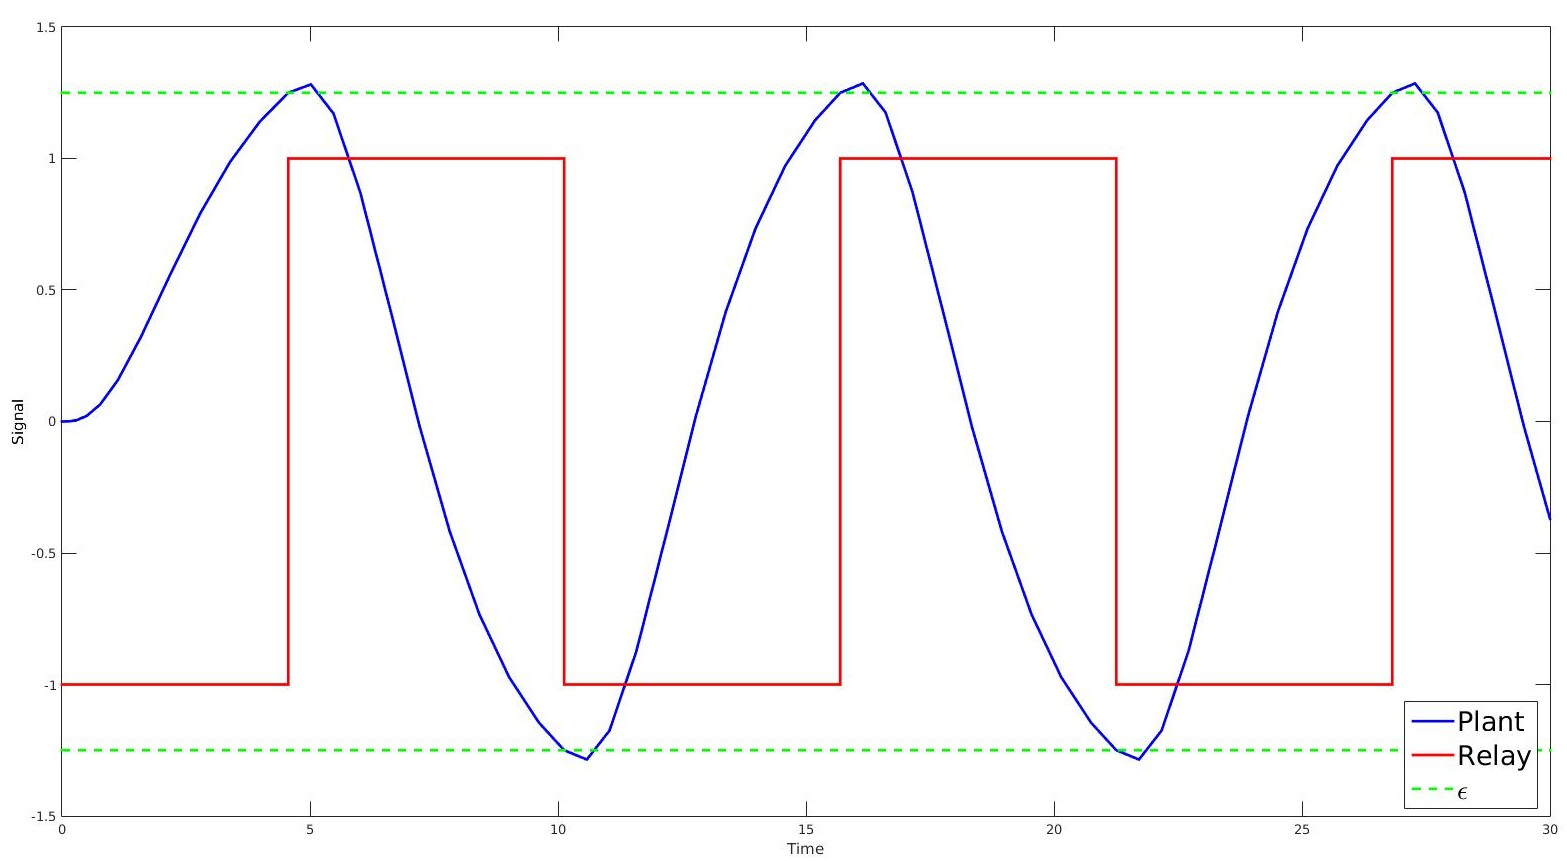
\includegraphics[width = 0.8\textwidth]{simple_relay_feedback.jpg}
\caption{Oscillations in a relay feedback system. The relay switches when the plant reaches the hysteresis limits $\pm \epsilon$, causing the plant to oscillate between those limits.}
\label{relay_feedback_oscillations}
\end{figure}
\color{black}


Figure \ref{relay_feedback} reveals how a typical relay feedback system is connected. The output of a plant ($y$), is connected to the relay ($e = -y$), and the output of the relay is input to the plant. Relay feedback systems tend to cause oscillations as the plant is subjected to maximal input (high or low) in the opposite direction when the plant exceeds a threshold ($\epsilon$ or $-\epsilon$), as shown in  Figure \ref{relay_feedback_oscillations}.

Relay feedback systems combine analogue and digital signals and can thus model switching behaviour in biological oscillations.

\subsection{Symmetric oscillations}
Consider the linear time invariant system:
\begin{eqnarray}
\begin{array}{l}
\displaystyle \dot{x} = Ax + Bu \\
\displaystyle y = Cx \\
\end{array}
\label{LTIsystem}
\end{eqnarray}

When this system is connected to the relay \ref{eq:symmetric_relay_equation}, with $e = -y$, the system can have a symmetric limit cycle of period $T=2h$ if the following condition is met:
\begin{equation}
C(I+e^{Ah})^{-1}\int_0^he^{As}B\text{d}s = \tfrac{\epsilon}{d}
\label{eq:2_3}
\end{equation}

\subsection{Asymmetric oscillations}\label{sec:asymm_oscillations}

When the relay is characterized by:

\begin{equation}
	u(t)=\begin{cases}
	               d_1 \text{ if } e > \epsilon \text{ or } (e >-\epsilon \text{ and } u(t-) = d_1)\\
	                -d_2 \text{ if } e < -\epsilon \text{ or } (e < \epsilon \text{ and } u(t-) = -d_2)\\
	              
	            \end{cases}
                \label{asymmetric_relay_equation}
\end{equation}

The LTI system given by (\ref{LTIsystem}) can have asymmetric oscillations when $e=-y$ and the following conditions for a limit cycle with period $T$ are met:
\begin{equation}
\begin{cases}
C(I-\Phi)^{-1}(\Phi_2\Gamma_1d_1-\Gamma_2d_2) = -\epsilon \\
C(I-\Phi)^{-1}(-\Phi_1\Gamma_2d_2+\Gamma_1d_1) = \epsilon \\
\end{cases}
 \label{eqtn5_2}
\end{equation}
where
\begin{equation}
\begin{array}{l}
\displaystyle \Phi = e^{AT}  \text{  ,  }\Phi_1 = e^{A\tau} \text{  ,  }  \Phi_2 = e^{A(T-\tau)} \\
\displaystyle \Phi_1 = \int_0^\tau e^{As}\text{d}sB \text{  ,  } \Gamma_2 = \int_0^{T-\tau}e^{As}\text{d}sB
\end{array}
\end{equation}
The asymmetric oscillation is split into two parts, a period when the relay output is low, $\tau$ and the period when the relay output is high, $T-\tau$, as shown in Figure \ref{fig:asym_relay_oscillations}.

\begin{figure}
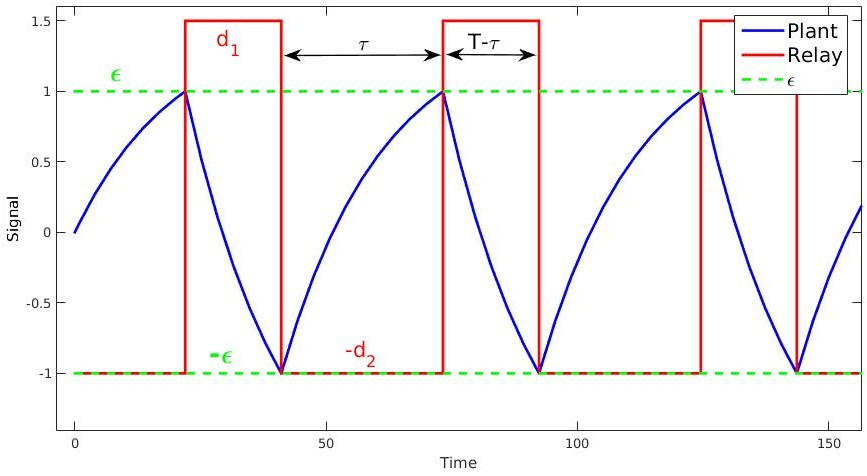
\includegraphics[width = 0.8\textwidth]{asym_relay_feedback}
\caption{Asymmetric oscillations with relay feedback.}
\label{fig:asym_relay_oscillations}
\end{figure}

In this project, once a model was approximated using relay feedback, the tools given stated above were used to predict the existence of limit cycles and their time periods. Parameters of a model could be varied and their effect understood by the above equations. \cite{astrom1995} also derived initial conditions for these oscillations and how to check the local stability of the oscillations.

\FloatBarrier
\section{Relay feedback models of fundamental biological limit cycles}\label{Sec:continous oscillations}
Two fundamental models of continuous oscillations in biology will be modelled as relay feedback systems in this section. This step reveals the use of relay feedback in order to predict time periods of oscillations and understanding how different parameters affect oscillations. 

\subsection{Goodwin oscillator model}
The Goodwin oscillator is a biochemical oscillator based on negative feedback alone. This genetic oscillator  describes the mechanism of how mRNA, protein and end product interact. Written in their non-dimensional form \cite{fall}, the Goodwin oscillator's kinetic equations are:
\begin{align}
\frac{dx_1}{dt'} &= \frac{1}{1 + x_3^p} - b_1x_1 \\
\frac{dx_2}{dt'} &= b_2(x_1 - x_2) \\
\frac{dx_3}{dt'} &= b_3(x_2 - x_3)
\end{align}
where $x_1,x_2.x_3$ are non-dimensionalised concentrations of mRNA, protein and end product, respectively. 
\noindent The only nonlinearity, $(\frac{1}{1 + x_3^p})$, becomes a relay with no hysteresis as $p \rightarrow \infty$ (see Figure \ref{goodwin_nonlinearity}).

\begin{figure}[h!]
\centering
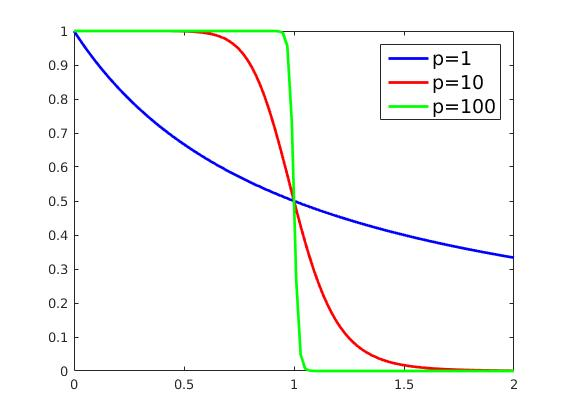
\includegraphics[width=0.5\textwidth]{goodwin_nonlinearity.jpg}
\caption{Nonlinearity becomes a relay with no hysteresis, as $p \rightarrow \infty$.}
\label{goodwin_nonlinearity}
\end{figure}
\begin{figure}[h!]
\centering
%\resizebox{6cm}{!}{%
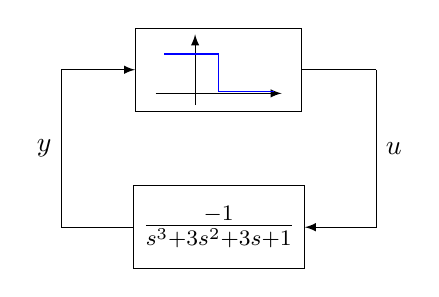
\begin{tikzpicture}[auto, node distance=2cm,>=latex]
\tikzstyle{block} = [draw,  rectangle,  minimum height=3em, minimum width=6em]
\tikzstyle{sum} = [draw,  circle, node distance=1cm]
\tikzstyle{input} = [coordinate]
\tikzstyle{output} = [coordinate]
\tikzstyle{pinstyle} = [pin edge={to-,thin,black}]   % We start by placing the blocks

\def\relay{
\tikz[remember picture,overlay]{
\draw[->] (-.8,-.3) -- (.8,-0.3);
\draw[->] (-.3,-0.45)--(-.30,0.45);
\draw[blue] (0.7,-0.28)--(0.,-0.28)--(0,0.2)--(-.7,.2);
%\draw[blue] (-.2,.2)--(-.2,-.2)--(.2,-.2);
}}

    \node [block] (inverse) {};
    \node[] at (inverse) {\relay};
    \node [output, right of = inverse] (output) {};
    \node [input, left of = inverse](input){};
    \node [block, below of = inverse](linear_tf){\large $\frac{-1}{s^3 + 3s^2 + 3s + 1}$};

    % Once the nodes are placed, connecting them is easy. 
    \draw [-] (inverse) -- (output);
    \draw [->] (output) |- node[near start] {$u$}(linear_tf);
    \draw [-] (linear_tf) -| node[near end] {$y$} (input);
    \draw [->] (input) -- (inverse);

\end{tikzpicture}
%}
\caption{Relay feedback system model of Goodwin oscillator ($b_1=b_2=b_3=1$). }
\label{goodwin_transfer}
\end{figure}

Setting $b_1 = b_2 = b_3 = 1$ (for simplicity) and rewriting the equations such that the linear equations form the plant and the nonlinearity is a relay, results in the system shown in Figure \ref{goodwin_transfer} with state space realisation: 
\begin{align}\label{eq:goodwin_relay_state_space}
\dot{x} &= \begin{bmatrix}
-1 & 0 & 0 \\  1  & -1 & 0 \\ 0 & 1 & -1
\end{bmatrix}x + \begin{bmatrix}1 \\0 \\0 \end{bmatrix}u \\
y &= \begin{bmatrix} 0 & 0 & 1 \end{bmatrix} u\\
u &=\begin{cases} 	               0 \text{ if } e \geq 1)\\
	                1 \text{ if } e < 1)\\\end{cases}
\end{align}

Using the theory for asymmetric oscillations, initial conditions were derived numerically. The limit cycle with the appropriate time period was shown to be locally stable and the simulations of the Goodwin model (with a very large $p$) and the relay feedback model were very similar (see Figure \ref{goodwin_matching}). This (novel) use of relay feedback systems to model biological oscillations is a link between classical control theory and biological models. The relay feedback model of gene dynamics explicitly models the logic of a gene turning off/on, and gives new insight into understanding these oscillations. 

\begin{figure}[h!]
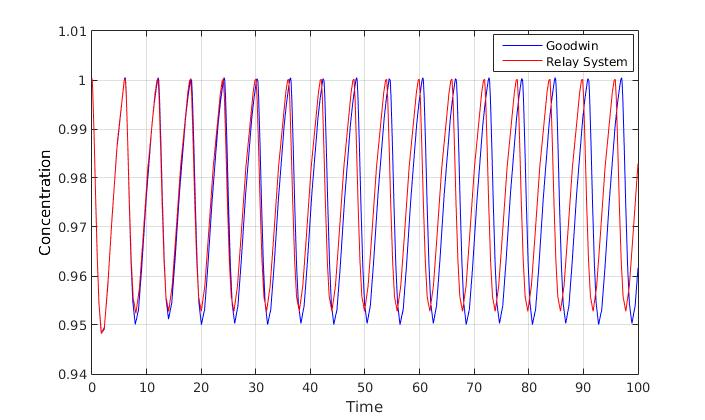
\includegraphics[width = .8\textwidth]{goodwin_mathcing}
\caption{Relay system models Goodwin oscillator well as $p\rightarrow\infty$. The Goodwin model had $p = 99999999$. This led to the model being very `stiff', with Matlab's \texttt{ode23tb} solver giving the best results.}
\label{goodwin_matching}
\end{figure}

\FloatBarrier
\subsection{FitzHugh-Nagumo model}
In this section, the use of relay feedback systems is extended to model a system where the relay is not as `obvious', as was in the previous section.
\subsubsection{Introduction}
The Hodgkin-Huxley model was the first quantitative model of the propagation of an electrical signal along a squid giant axon \cite{keener}. It is the most important model in all of the physiological literature \cite{keener}, and led to the study of excitable systems.  The FitzHugh-Nagumo model simplifies the Hodgkin-Huxley model (of four variables) in terms of two variables, one fast and one slow. With the fast variable, $v$, representing the voltage and the slow variable, $w$, representing the current, the FitzHugh-Nagumo model is:
\begin{align}
\epsilon\dot{v} &= f(v) - w + I_\text{app}\\
\dot{w} &= v - \gamma w
\end{align}
where: 
\begin{equation*}
\epsilon \ll 1 \text{  and  } f(v) = v(1-v)(v-\alpha) \text{ , } 0 <\alpha<1 .
\end{equation*} 
$I_\text{app}$ is the externally applied current (representing the stimulus). The nullclines\footnote{The nullcline is the line along which a variable's time derivative is zero} of the fast and slow variables have a cubic shape and a linear shape respectively.   The input current, $I_\text{app}$, shifts the cubic nullcline, affecting where the nullclines intersect, i.e the equilibrium points. For certain input currents, the nullclines intersect at only one (unstable) point and cause continous oscillations. With $\alpha =0.1, \gamma = 0.5, \epsilon = 0.01$ and $I_{\text{app}}=0.5$, the uniqure rest point is unstable. Since $\epsilon \ll 1 $, the fast variable tries to follow the stable branches of the cubic nullcline where possible and then quickly jumps to the other stable branch. That is the voltage stays at a high value for some time and then quickly jumps to a low value and then jumps up to a high value (see Figure \ref{fig:FN_intro}).  Meanwhile, the current slowly adapts to the high/low value of the voltage, pushing the system to leave the stable branches eventually. The behaviour of the system in the phase plane follows from singular perturbation theory\cite{keener}. 

\begin{figure}
\centering
    \begin{subfigure}[b]{0.45\textwidth}
        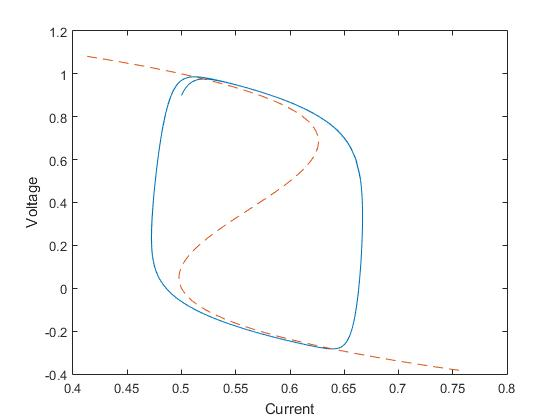
\includegraphics[width=\textwidth]{fitz_nagumo_hysteresis.jpg}
        \caption{Phase portrait. The cubic nullcline is shown as the dashed line.}
        \label{fig:FN_intro_hysteresis}
    \end{subfigure}
    ~ %add desired spacing between images, e. g. ~, \quad, \qquad, \hfill etc. 
      %(or a blank line to force the subfigure onto a new line)
    \begin{subfigure}[b]{0.45\textwidth}
        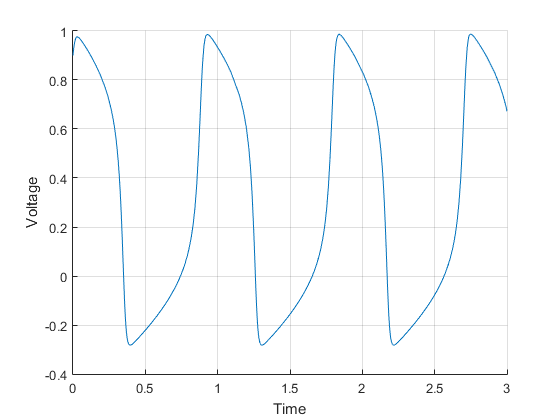
\includegraphics[width=\textwidth]{fitz_nagumo_voltage_time.png}
        \caption{Voltage oscillations.}
        \label{fig:FN_intro_voltage}
    \end{subfigure}
    \caption{Continous oscillations in the FitzHugh-Nagumo model.}
    \label{fig:FN_intro}
\end{figure}

\begin{figure}
\centering
    \begin{subfigure}[b]{0.45\textwidth}
        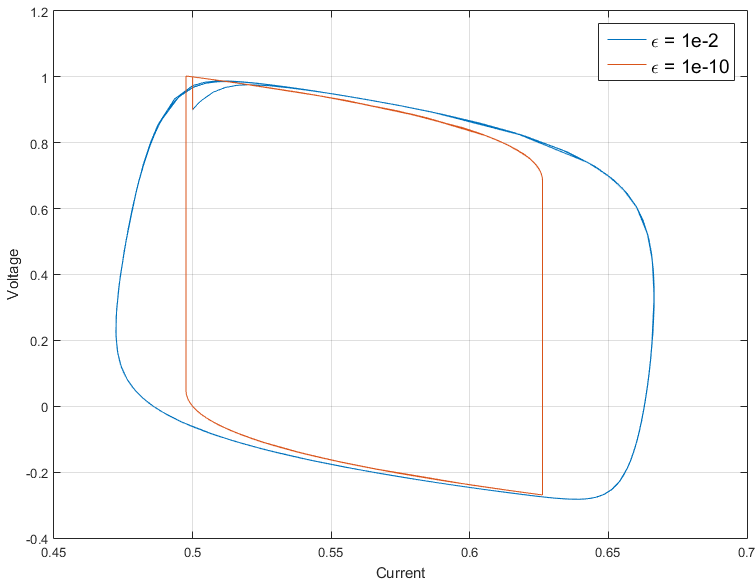
\includegraphics[width=\textwidth]{fitz_nagumo_speed}
        \caption{Phase portrait. Hysteresis becomes more linear and `relay'.}
        \label{fig:FN_eps_hysteresis}
    \end{subfigure}
    ~ %add desired spacing between images, e. g. ~, \quad, \qquad, \hfill etc. 
      %(or a blank line to force the subfigure onto a new line)
    \begin{subfigure}[b]{0.45\textwidth}
        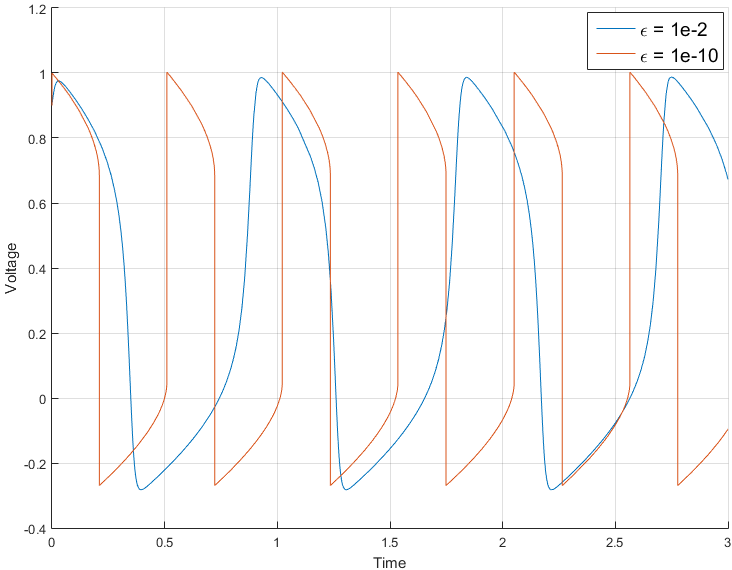
\includegraphics[width=\textwidth]{fitz_nagumo_speed_voltage_time.png}
        \caption{Voltage oscillations become more `discrete', similar to a relay ouput.}
        \label{fig:FN_eps_voltage}
    \end{subfigure}
    \caption{In the limit $\epsilon\rightarrow0$, the voltage ouput looks like the output of a relay. The hysteresis looks like a skewed relay. }
    \label{fig:FN_eps_zero}
\end{figure}

\subsubsection{Converting to relay feedback model}\label{sec:FN_to_relay}

As $\epsilon\rightarrow 0$, the phase portrait of the voltage and current becomes more and more linear and closely resembles a rotated relay with hysteresis (Figure \ref{fig:FN_eps_zero}. This can be understood as  high gain inversion \cite{goodwin}, and the voltage behaves like the ouput of a skewed relay. So, when the system is coninously oscillating, it allows one to replace the cubic nullcline with a skewed relay. 

\begin{figure}[h!]
\begin{subfigure}[t]{.4\textwidth}

\centering
\tikzstyle{block} = [draw,  rectangle,  minimum height=3em, minimum width=6em]
\tikzstyle{sum} = [draw,  circle, node distance=1cm]
\tikzstyle{input} = [coordinate]
\tikzstyle{output} = [coordinate]
\tikzstyle{pinstyle} = [pin edge={to-,thin,black}]
\resizebox{5cm}{!}{%
  % The block diagram code is probably more verbose than necessary
  \begin{tikzpicture}[auto, node distance=2cm,>=latex,scale=0.75]
      % We start by placing the blocks
      \node at (0,3) (I_app) {$I_{app}$};
      %\node[input, name = I_app]{text};
      \node[sum, right of = I_app](sum_outer){};
      \node [sum, right of = sum_outer] (sum_inner) {};
      \node [block, right of = sum_outer, node distance=3cm] (high_gain) {\large{$\frac{1}{\epsilon s}$}};
      % We draw an edge between the controller and system block to 
      % calculate the coordinate u. We need it to place the measurement block. 
      \node [output, right of = high_gain] (output) {};
      \node [block, below of = high_gain] (cubic_nullcline) {$f(\cdot)$};
      \node [block, below of = cubic_nullcline](linear_tf){\large $\frac{1}{s+\gamma}$};

      % Once the nodes are placed, connecting them is easy. 

      % inner loop
      \draw [draw,->] (sum_outer) -- node {$+$} (sum_inner);
      \draw [->] (sum_inner) -- node {$\dot{v}$} (high_gain);
      \draw [->] (high_gain) -- node [name=v] {$v$}(output);
      \draw [->] (v) |- (cubic_nullcline);
      \draw [->] (cubic_nullcline) -| node[pos=.85] {$+$} 
          node [near end] {} (sum_inner);

      % outer loop
      \draw [->](v) |- (linear_tf);
      \draw [->](linear_tf) -| node[anchor=south,pos=0.2] {$w$} 
          node[pos=0.93]{-}(sum_outer);
      \draw [->](I_app)-- node[near end]{$+$} (sum_outer);
  \end{tikzpicture}}
	\caption{Block diagram}%
	\label{fitz_nagumo_block_diagram1}%
\end{subfigure}
\hspace{0.5cm}%
\begin{subfigure}[t]{.45\textwidth}
\centering
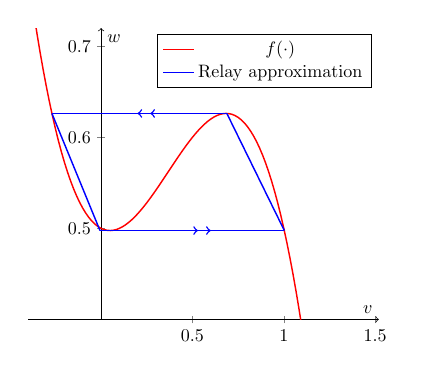
\begin{tikzpicture}[scale = 0.65]
  \begin{axis}[
    xmin=-.4,xmax=1.52,
    ymin=0.4,ymax=.72,
    axis lines=center,
    axis line style=->,
    xlabel={$v$},
    ylabel={$w$}
    ]
      \addplot[-] [color=red, style = thick] expression[domain=-0.45:1.2,samples=100]{-x^(3)+(1+0.1)*x^(2) - 0.1*x + 0.5}; 
      \addplot[-] [color=blue, style = thick] coordinates{(-.2693,0.6262) (.6883,.6262)};
            \addplot[<-] [color=blue, style = thick] coordinates{(.2693,0.6262) (.6883,.6262)};
            \addplot[<-] [color=blue, style = thick] coordinates{(.1993,0.6262) (.6883,.6262)};
      \addplot [color=blue, style = thick] coordinates{(.6883,0.6262) (1.003,.4976)};
      \addplot [color=blue, style = thick] coordinates{(-.2693,0.6262) (-.0061,.4976)};
      \addplot [-][color=blue, style = thick] coordinates{(-.0061,.4976) (1.003,.4976)};
      		\addplot [->][color=blue, style = thick] coordinates{(-.0061,.4976) (.6,.4976)};
            \addplot [->][color=blue, style = thick] coordinates{(-.0061,.4976) (.53,.4976)};
     % \addplot[-] [color=green, style = thick] expression[domain=-0.45:1.2,samples=100]{-y^(3)+(1+0.1)*y^(2) - 0.1*y + 0.5}; 
     \addlegendentry{$f(\cdot)$}
	 \addlegendentry{Relay approximation}
	\end{axis}
\end{tikzpicture}
	\caption{Nonlinearity and the ``relay" approximation}%
	\label{original_nonlinearity1}%
\end{subfigure}
\caption{FitzHugh-Nagumo model.}
\label{fn}
\end{figure}


\underline{High gain inversion}
\begin{align}
0 &= f(v) -w + I_{\text{app}}\\
v &= f^{-1}\left(w - I_{\text{app}}\right)\\
v&\approx \text{Relay}(w) 
\end{align}

This allows us to replace the inner loop in \ref{fitz_nagumo_block_diagram1}. With a shift in co-ordinates to make the `relay' symmetric about the orgin, and a change of basis so that an unskewed relay can be used, results in the relay feedback system in Figure \ref{fig:fitz_nagumo_relay_block_diagram}. Details of this transformation are illustrated in the Appendix. Now, using \ref{eq:2_3}, we can derive the time period of the oscillation and its local stability. The results are shown in Figure \ref{fig:matching_fitz_relay}. The relay feedback model matches the oscillations very closely. 

This model reveals how the oscillations can be understood as adaptation around a hysteresis. The current slowly adapts to each change in voltage, around the relay hysteresis, causes the voltage to oscillate. 

\begin{figure}[h!]

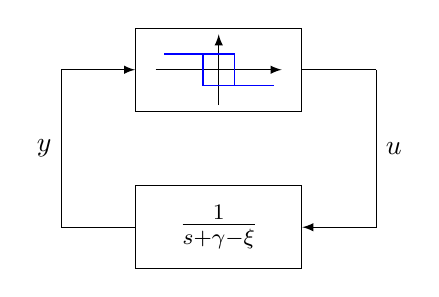
\begin{tikzpicture}[auto, node distance=2cm,>=latex, scale = 0.25]
\tikzstyle{block} = [draw,  rectangle,  minimum height=3em, minimum width=6em]
\tikzstyle{sum} = [draw,  circle, node distance=1cm]
\tikzstyle{input} = [coordinate]
\tikzstyle{output} = [coordinate]
\tikzstyle{pinstyle} = [pin edge={to-,thin,black}]   % We start by placing the blocks

\def\relay{
\tikz[remember picture,overlay]{
\draw[->] (-.8,0) -- (.8,0);
\draw[->] (0,-0.45)--(0,0.45);
\draw[blue] (0.7,-0.2)--(0.2,-0.2)--(0.2,0.2)--(-.7,.2);
\draw[blue] (-.2,.2)--(-.2,-.2)--(.2,-.2);
}}

    \node [block] (inverse) {};
    \node[] at (inverse) {\relay};
    \node [output, right of = inverse] (output) {};
    \node [input, left of = inverse](input){};
    \node [block, below of = inverse](linear_tf){\large $\frac{1}{s+\gamma-\xi}$};

    % Once the nodes are placed, connecting them is easy. 
    \draw [-] (inverse) -- (output);
    \draw [->] (output) |- node[near start] {$u$}(linear_tf);
    \draw [-] (linear_tf) -| node[near end] {$y$} (input);
    \draw [->] (input) -- (inverse);

\end{tikzpicture}
\caption{Relay feedback model of FitzHugh-Nagumo.}
\label{fig:fitz_nagumo_relay_block_diagram}
\end{figure}

\begin{figure}[h!]
    \centering
    \begin{subfigure}[t]{0.45\textwidth}
        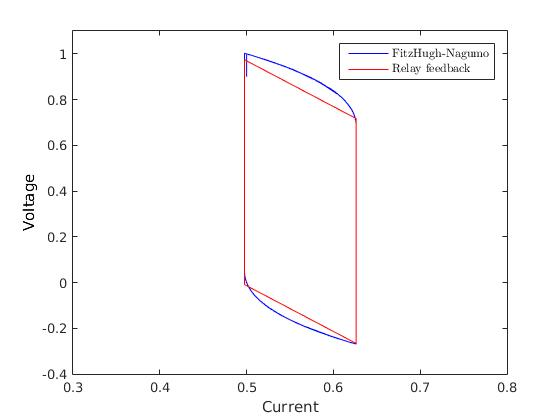
\includegraphics[width=\textwidth]{tmr_fn_relay_limit_cycle}
        \caption{Phase Portrait. Voltage is like the output of a skewed relay.}
        \label{fig:f_n_relay_limit_cycle}
    \end{subfigure}
    ~ %add desired spacing between images, e. g. ~, \quad, \qquad, \hfill etc. 
    %(or a blank line to force the subfigure onto a new line)
    \begin{subfigure}[t]{0.45\textwidth}
        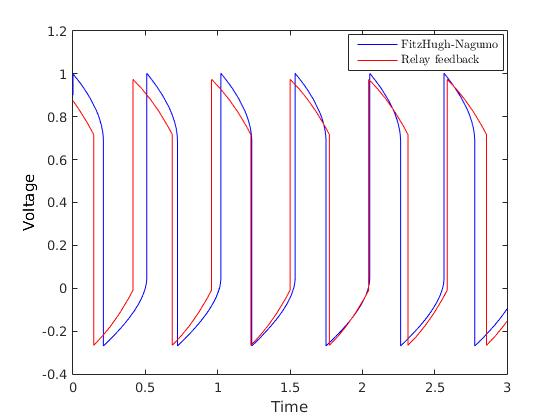
\includegraphics[width=\textwidth]{tmr_fn_relay_voltage}
        \caption{Voltage oscillations against time. Voltage alternates between a high state and a low state.}
        \label{fig:f_n_relay_voltage}
    \end{subfigure}
\caption{FitzHugh-Nagumo model and Relay feedback model match in $\lim\limits_{\epsilon\to 0}$}
\label{fig:matching_fitz_relay}
\end{figure}

\FloatBarrier


\section{Relay feedback model of nested oscillations}\label{Sec:nested oscillations}
In this section, the application of the use of relay feedback analysis is extended to a more complex biological oscillation --- bursting. A bursting model's nonlinearities are simplifed to piecewise-linear non-linearites and a separation of time scales approach is used to decompose the two coupled oscillators. 

\subsection{Bursting}
Bursting is an important signaling component of neurons, characterized by a periodic alternation of bursts (periods of rapid oscillatory activity) and quiescent (membrane potential changes slowly)periods\cite{franci2}. Bursting observed in cells can have a wide variety of periods, ranging from a few seconds to a few minutes \cite{keener}. This general phenomenon is believed to play an important role in several signalling mechanisms. Bursting can also be viewed as a two state automaton in frequency. It can encode memory into four states-- resting, fast oscillations, slow oscillations and bursting. 

All neuronal bursters have three distinct time scales: a fast time-scale for spike generation, a slow time-scale for the intraburst spike frequency, and an ultra slow time-scale for the inter burst frequency\cite{franci2}. This sepration of timescales is used to decompose bursting into two coupled relay feedback systems. As a first step, the bursting model from \cite{franci} is introduced. Then, the nonlinearites are simplified and finally, the three different time scales are separated out to reduce the model into relay feedback systems. 

\subsection{Three-time scale bursting attractor}
The three-time scale bursting attractor organized by the winged cusp is a bursting model presented in \cite{franci}. It is based on unfolding of the organizing center called the winged cusp to obtain a finite family distinct,robust static behaviours \cite{franci}. The model is based on Singularity theory and the interested reader is referred to \cite{franci} for a comprehensive exposition of how this model realises a variety of nonlinear behaviours. 

The fundamental basis for this model is the robust co-existence of a stable fixed point and a stable relaxation limit cycle as shown in Figure\ref{fig:bursting_fundamental_phase_portait}. The stable limit cycle is similar to the FitzHugh-Nagumo model's phase portrait. This model generalizes FitzHugh-Nagumo by adding a third variable (ultra-slow)  in negative feedback, which adapts in the dimension normal to the phase portrait (see Figure \ref{fig:3d_bursting}). This adaptation switches the behaviour between spiking and resting. The state-space equations for this model is:
\begin{equation}
\begin{array}{l}
\displaystyle \epsilon_f\dot{x}_{f} = -x_f + S\left(x_f + B_\delta\left(u + x_s + \tfrac{\gamma}{2}x_f\right) + \beta x_f + \alpha  - x_{us}  \right)\\
\displaystyle \dot{x}_{s} = x_f - x_s \\
\displaystyle \dot{x}_{us} = \epsilon_u\left(-x_{us} + k_u(x_f+\bar{x}_u) \right)\\
\end{array}
\label{eq:restSpikeBistability}
\end{equation}
where:
\begin{equation}
\begin{array}{l}
\displaystyle \text{Sigmoid nonlinearity: }S(u) = \text{tanh}(u) \\
\displaystyle \text{Bump nonlinearity: }B_\delta(u) := S(u+\delta) - S(u-\delta) -2S(\delta),\hspace{0.4cm} \delta\neq0
\end{array}
\end{equation}


\begin{figure}[h!]
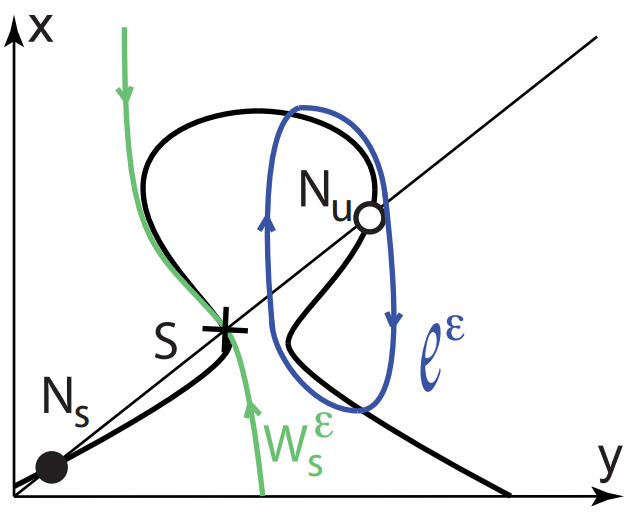
\includegraphics[width = 0.5\textwidth]{winged_cusp_phase_portrait}
\caption{Phase portrait (qualitative) of the three-time scale bursting attractor. $N_s$ is the stable equilibrium, $N_u$ is the unstable equilibrium, $S$ is the saddle point, $W_s^\epsilon$ is the stable manifold of $S$ and $l^\epsilon$ is a stable limit cycle. The thick black line is the fast variable's nullcline, known as the mirrored hysteresis (winged cusp singularity) and the slow variable's nullcline is the thin straight line. Source \cite{franci2}.}
\label{fig:bursting_fundamental_phase_portait}
\end{figure}

\begin{figure}
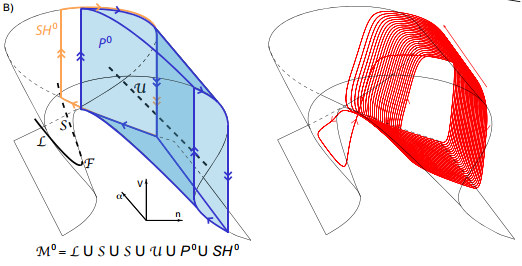
\includegraphics[width = 0.7\textwidth]{franci_3d_bursting}
\caption{Three-dimensional singular invariant set $\mathcal{M}^0$ (left), which provides a skeleton for a three-time scale bursting attractor (right). The ultra-slow parameter adapts to swtich the system from spiking to resting and vice versa. See \cite{franci2} Figure 4 for details. Source \cite{franci2}.}
\label{fig:3d_bursting}
\end{figure}

The block diagram for this circuit is shown in Figure \ref{fig:ttsbursting_circuit}. Typical bursting is shown in Figure \ref{fig:bursting_typical_oscillations} where the ultra-slow variable modulates the behaviour.

\begin{figure}
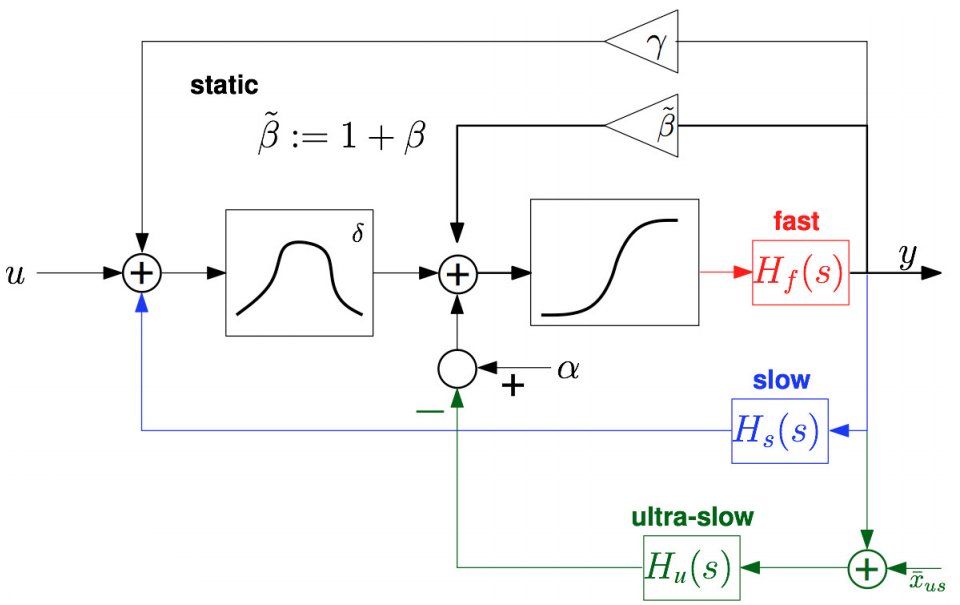
\includegraphics[width = 0.5\textwidth]{tts_circuit}
\caption{Three-time scale bursting acctractor block diagram. Source \cite{franci}.}
\label{fig:ttsbursting_circuit}
\end{figure}

 \begin{figure}
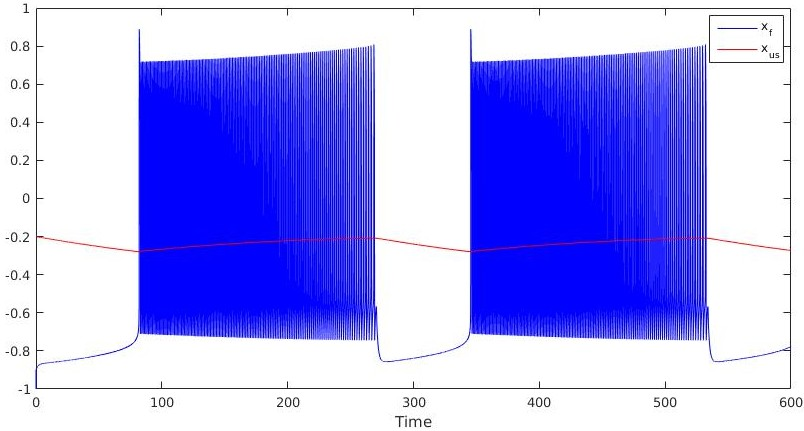
\includegraphics[width = 0.8\textwidth]{original_bursting.jpg}
\caption{Bursting. The ultra-slow oscillations of the $x_{us}$ switches the output $x_f$ between spiking and resting.}
\label{fig:bursting_typical_oscillations}
\end{figure}



\subsubsection{The adaptation parameter for the ultra-slow negative feedback loop }
The (unfolding) parameter $\alpha$ modulates monotonically the winged-cusp singularity\cite{franci}, as shown in Figure \ref{fig:alphaParameter}. The bursting model thus relies on continously adapting this parameter, using the ultra-slow variable, around the bistable range. As $x_{us}$ reaches its maximum value, the nullclines of the fast and slow variables will only intersect at the stable fixed point (low $x_f$). This drives the system to the quiescent period, while $x_{us}$ slowly recovers. When $x_{us}$ reaches its minimum value, the nulclines of the fast and slow variables will only intersect at a high $x_{us}$ which then becomes the unstable fixed point as $x_{us}$ recovers. This drives the system to the spiking period. 
It is clear now that the ultra-slow parameter can be modelled as a relay feedback system, oscillating around the bistable range. However, due to the bump nonlinearity, the slow and fast systems need some more dissection before it can be modelled as a relay feedback system.



\begin{figure}
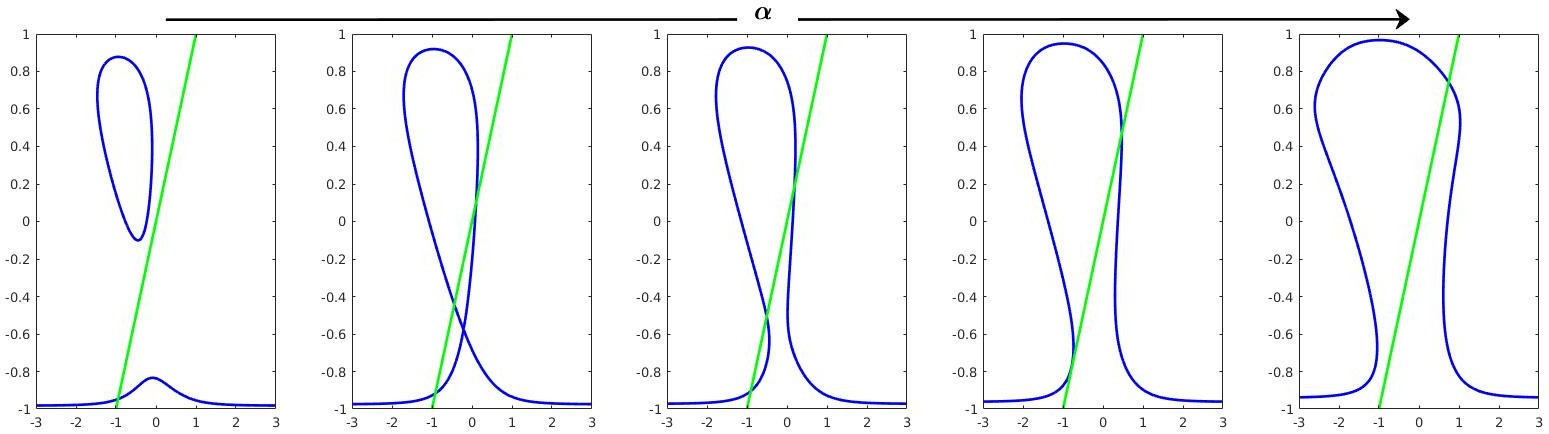
\includegraphics[width = 0.9\textwidth]{restSpikeBistableAlpha}
\caption{Fast nullcline changing as $\alpha$ increases. Within a fixed range of $\alpha$, the system has both the resting and the spiking equilibrium. This is the bistable range.}
\label{fig:alphaParameter}
\end{figure}
\FloatBarrier
\subsubsection{The positve feedback in fast inner loop}
The positive feedback of the fast plant around the sigmoidal nonlinearity creates a nonlinearity with hysteresis. This can be understood by considering positive feedback for a saturation function, shown in Figure \ref{fig:positive_feedback_hysteresis}. By assuming that $x_f$ is much faster than the other variables, we can clearly approximate the positve feedback loop as a relay. This is equivalent to $\epsilon_f\rightarrow 0$, which was done earlier for the FitzHugh-Nagumo model. 

\begin{figure}
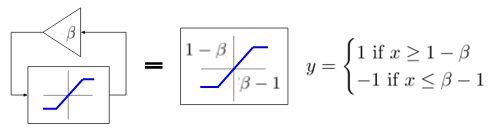
\includegraphics[width = 0.7\textwidth]{positive_feedback_hysteresis}
\caption{For the saturation function, for $\beta > 1$, the nonlinearity gains a hysteresis of width $2\beta$. }
\label{fig:positive_feedback_hysteresis}
\end{figure}

\subsubsection{The bump nonlinearity}
The bump nonlinearity (Figure \ref{fig:bump_nonlinearity}) affects what kind of feedback the slow plant provides. When the system is spiking, the input to the bump is always greater than zero. This means the system was in the regime where the bump had a negative gradient. The bump provided negative feedback, causing the slow plant to adapt around the hysteresis of the sigmoid nonlinearity. That is, when spiking, the model essentially simplifies down to the FitzHugh-Nagumo model during continous oscillations. However, when the model was quiescent, the input to the bump was negative. The bump provided positive feedback, driving the system to the stable equilibrium. 

Now it is required to simplify this model in order to allow us to use the analytical results for relay feedback systems.

\begin{figure}
\begin{tikzpicture}[auto, node distance=2cm,>=latex, scale = 1]
\draw [fill = white](1,1) rectangle (10,7);
\end{tikzpicture}
\caption{Bump nonlinearity}
\label{fig:bump_nonlinearity}
\end{figure}
\FloatBarrier
\subsection{Using piece-wise linear non-linearities}
As shown in \ref{fig:sigmoid_linear}, the saturation function is a good approximation to the sigmoidal nonlinearity. Furthermore, since the positive feedback gain is $\tilde{\beta}:=1 + \beta$, this can be replaced by a positive feedback of just $\beta$ around a relay with no hsyteresis. The is then equivalent to a relay with hysteresis limits $\pm \beta$. 

\begin{figure}
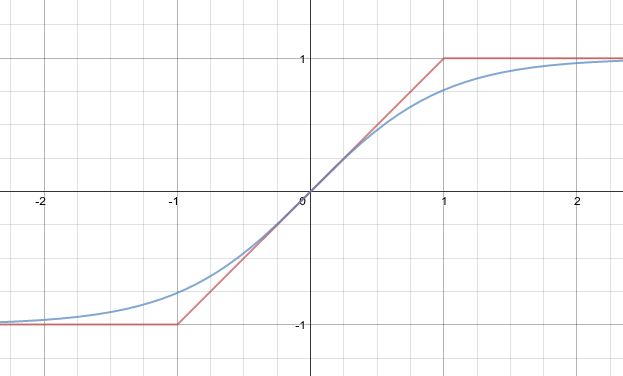
\includegraphics[width = 0.6\textwidth]{sigmoid_linear}
\caption{The $S(\cdot)$ and the saturation functions. The saturation function is a good approximation to the $S(\cdot)$. }
\label{fig:sigmoid_linear}
\end{figure}

The bump nonlinearity with $\delta$ set to 0.5, can be approximated by the piecewise linear function shown in Figure \ref{fig:bump_linear}. The piecewise linear function simplifies the model very nicely since the positive/negative feedback gain is constant. The function is:
\begin{equation}
B:= \begin{cases}
\frac{1}{2}x \text{ \hspace{3cm}  if } -2<x<0 \\
-\frac{1}{2}x \text{\hspace{3cm}if } 0<x<2 \\
-1 \text{ \hspace{3cm}  otherwise}
\end{cases}
\end{equation}

\begin{figure}
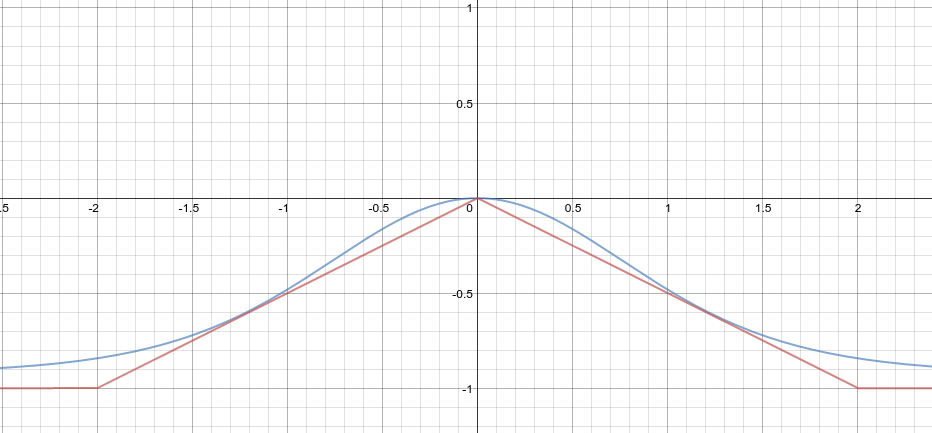
\includegraphics[width = 0.6\textwidth]{bump_and_linear}
\caption{The $B_\delta(\cdot)$ with $\delta = 0.5$ and a piecewise linear approximation.}
\label{fig:bump_linear}
\end{figure}

The system's phase portrait is shown in Figure \ref{fig:linearised_phase_portrait}. The new fast nullcline approximates the original nullcline. 

\begin{figure}
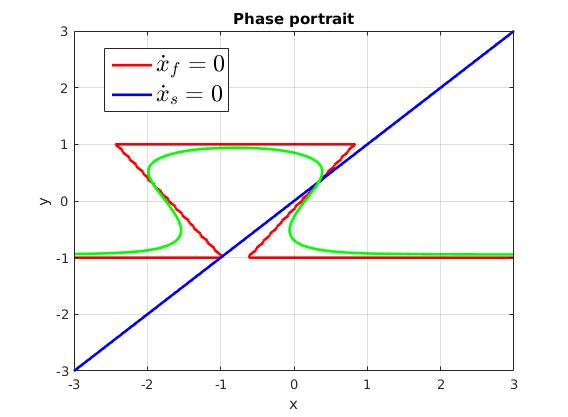
\includegraphics[width = 0.6\textwidth]{linearised_phase_portrait}
\caption{Phase portrait using piecewise-linear nonlinearities. The original fast nullcline is plotted in green for comparison. Note that the lines showing $\dot{x}_f=0$ where $-1<x_f<1$ does not exist algebraicly. Numerical computing leads to those lines.}
\label{fig:linearised_phase_portrait}
\end{figure}

\subsection{Separation of time scales to separate into relay feedback systems}
By assuming that the fast variable changes instantaneously ($e_f\rightarrow0$), the innermost loop involving the fast plant $H_f$ can be replaced by a relay with hysteresis (Figure \ref{fig:bursting_step1}). 

\begin{figure}
\begin{tikzpicture}[auto, node distance=2cm,>=latex, scale = 1]
\draw [fill = white](1,1) rectangle (10,7);
\end{tikzpicture}
\caption{Inner loop replaced by relay with hysteresis}
\label{fig:bursting_step1}
\end{figure}

While the system is spiking, the bump nonlinearity can be replaced by a constant gain providing negative feedback. Furthermore, Figure \ref{fig:bursting_step2.1} shows how the ultra slow variable can be viewed as very slowly varying. This is equivalent to the relay feedback system with a slowly shifting hysteresis ( Figure \ref{fig:bursting_step2}). 

\begin{figure}
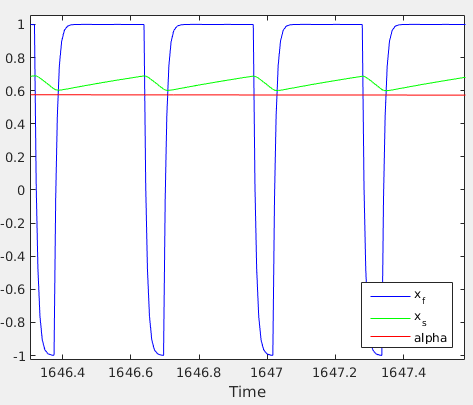
\includegraphics[width = 0.5\textwidth]{slow_fast}
\caption{Variables changing during a very short period of spiking. The slow variable is adapting around the static hysteresis, like in the FitzHugh-Nagumo model. The utra slow variable is changing very slowly.}
\label{fig:bursting_step2.1}
\end{figure}

\begin{figure}
\begin{tikzpicture}[auto, node distance=2cm,>=latex, scale = 1]
\draw [fill = white](1,1) rectangle (10,7);
\end{tikzpicture}
\caption{Relay feedback system with slowly shifting hysteresis.}
\label{fig:bursting_step2}
\end{figure}

Setting $\gamma = 0$ (without loss of generality), gives a hysteresis for the new system that is not skewed\footnote{Transformation for skewed hysteresis was carried out in Section \ref{sec:FN_to_relay}}. This allows us to use the analytical results from \cite{astrom1995} to predict the time periods of the oscillations. The shifting hysteresis limits, due to the ultra slow variable, change the time periods of the oscillations as shown in Figure \ref{fig:Tandtau}

\begin{figure}
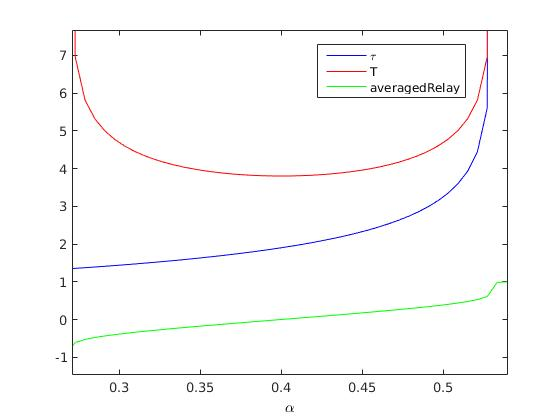
\includegraphics[width = 0.6\textwidth]{averagedRelay3}
\caption{Duty cycle of the spiking oscillations changing with the ultra slow variable.}
\label{fig:bursting_step2.1}
\end{figure}

The ultra-slow variable, due to its slow time constant, can be regarded as only responding to an ``averaged" $x_f$. Figures \ref{fig:bursting_step3.1} and \ref{fig:bursting_step3.2} reveal the response of $\alpha$ to a moving average $x_f$. The relay hysteresis limit is the bistable range of $\alpha$, while the maximum output of the relay can be roughly approximated as nearly zero. This reveals how the bursting circuit has been simplified into two coupled oscillators. The fast-slow oscillator which reproduces the spiking and the averge-fast--ultra-slow oscillator which dictates when the model spikes and rests (see Figure \ref{fig:bursting_step4}). 

\begin{figure}
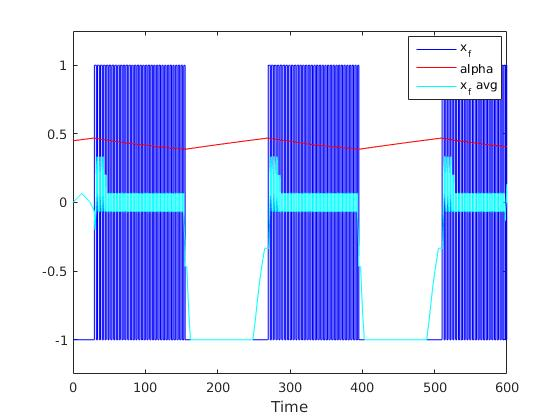
\includegraphics[width = 0.6\textwidth]{fastSlowaverg}
\caption{Moving average of $x_f$ changes during spiking as $\alpha$ changes the hysteresis limits.}
\label{fig:bursting_step3.1}
\end{figure}

\begin{figure}
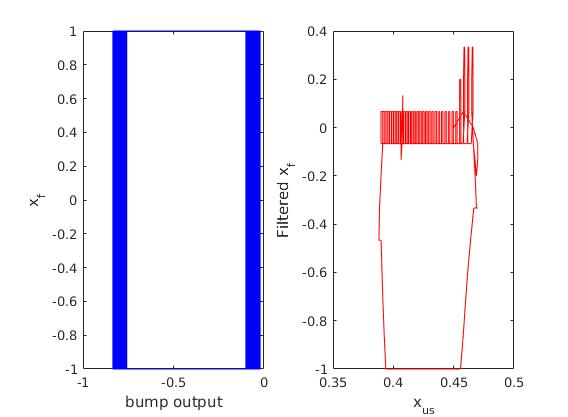
\includegraphics[width = 0.6\textwidth]{shiftinghysteresis}
\caption{Trajectories on the phase plane reveal shifting hysteresis for $x_f$ and an approximate relay hysteresis for $\alpha$}.
\label{fig:bursting_step3.2}
\end{figure}

\begin{figure}
\begin{tikzpicture}[auto, node distance=2cm,>=latex, scale = 1]
\draw [fill = white](1,1) rectangle (15,10);
\end{tikzpicture}
\caption{Coupled relay feedback systems.}
\label{fig:bursting_step4}
\end{figure}

The transforming of the three time scale burster into relay feedback models now enables us to analytically extract the time period of the slow oscilaltion and that of the fast oscillation. It also revealed how the two oscillators are linked and revealed how the duty cycle during spiking sublty changes due to the ultra-slow parameter. 

\FloatBarrier
\subsection{Hindmarsh-Rose model}
The Hindmarsh-Rose model for bursting is a slight modification of the FitzHugh-Nagumo model for action potentials. It uses a parabolic nullcline for the slow variable instead of the a straight line. The model is below:
\begin{align}
\epsilon_f\dot{x}_f &= x_s -x_{us} + f(x_f) + I \\
\dot{x}_s &= g(x_f) - x_s\\
\dot{x}_{us} &= \tau_{us}\left(k(x_f-\bar{x}_{us}) - x_{us}\right)
\end{align}
with $f(x) = 3x^2 - x^3$ and $g(x) = 1 - 5x^2$. The fast variable $x_f$ represents the voltageFor bursting, the parameters used are $\tau_{us} = 0.001, k = 4, \bar{x}_{us} = 1.6, I = 2$. The behaviour of the model can be seen in Figure \ref{fig:hRose_bursting}

\begin{figure}[h!]
    \centering
    \begin{subfigure}[t]{0.48\textwidth}
        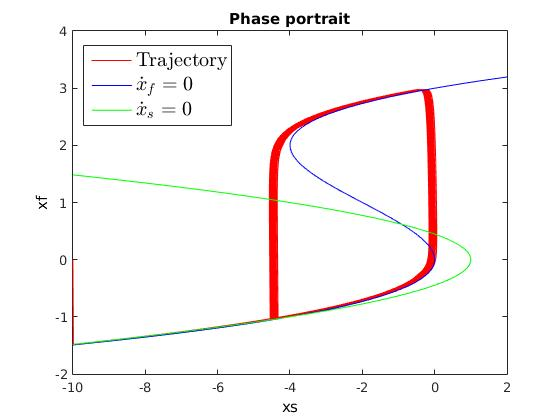
\includegraphics[width=\textwidth]{hRose_phase_portrait}
        \caption{Phase Portrait. Voltage is like the output of a skewed relay as $\epsilon_f\rightarrow0$, just like in the FitzHugh-Nagumo model.}
        \label{fig:hRose_phase_portrait}
    \end{subfigure}
    ~ %add desired spacing between images, e. g. ~, \quad, \qquad, \hfill etc. 
    %(or a blank line to force the subfigure onto a new line)
    \begin{subfigure}[t]{0.48\textwidth}
        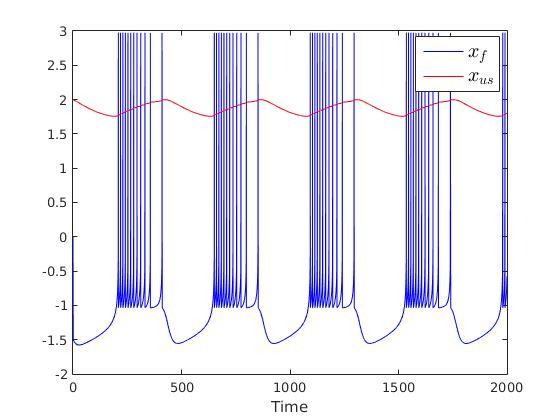
\includegraphics[width=\textwidth]{hRose_bursting}
        \caption{Voltage oscillations against time. Voltage alternates between a high state and a low state when spiking. It then moves to a lower state while resting.}
        \label{fig:hRose_voltage_time}
    \end{subfigure}
\caption{Hindmarsh-Rose model for bursting.}
\label{fig:hRose_bursting}
\end{figure}

In the same manner as the three-time scale bursting attractor, the ultra-slow negative feedback modulates the shape of the fast nullcline to change the equilibrium positions. This can be seen in Figure \ref{fig:hRose_changing_eqms}. 

\begin{figure}[h!]
    \centering
    \begin{subfigure}[t]{0.48\textwidth}
        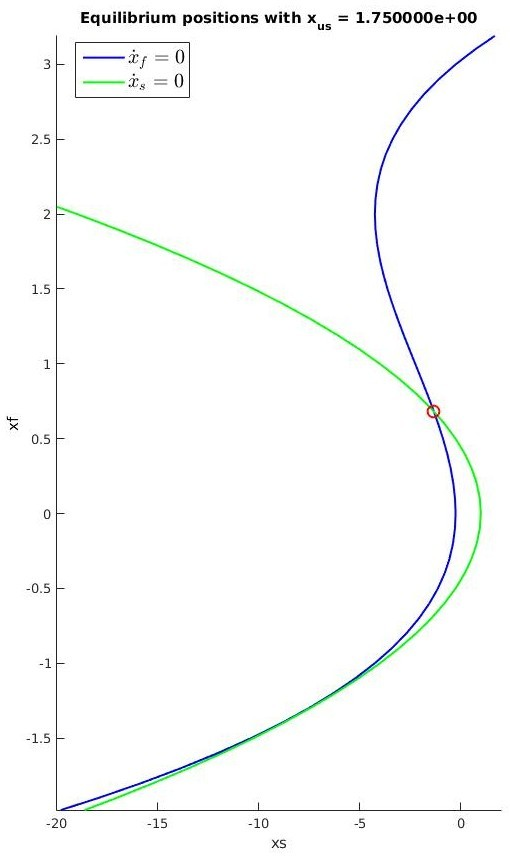
\includegraphics[width=\textwidth]{hRose_eqms1}
        \caption{The $x_{us}$ is just small enough that the nullclines interesect only once. The system will switch to spiking as this happens.}
        \label{fig:hRose_eqms1}
    \end{subfigure}
    ~ %add desired spacing between images, e. g. ~, \quad, \qquad, \hfill etc. 
    %(or a blank line to force the subfigure onto a new line)
    \begin{subfigure}[t]{0.48\textwidth}
        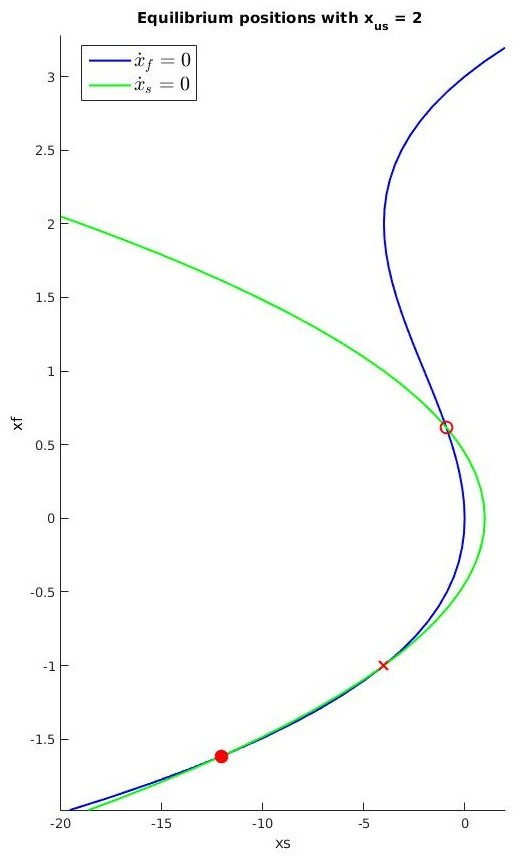
\includegraphics[width=\textwidth]{hRose_eqms2}
        \caption{The $x_{us}$ is just large enough that the nullclines interesect thrice. The system will switch to resting as this happens.}
        \label{fig:hRose_eqms2}
    \end{subfigure}
\caption{Fast nullcline of Hindmarsh-Rose model being modulated by the ultra-slow variable ($x_{us}$). Stable equilibrium is the filled circle, unstable equilibrium is the hollow circle and the saddle point is the cross. Between this range of $x_{us}$, the system is bistable.}
\label{fig:hRose_changing_eqms}
\end{figure}

\FloatBarrier
\section{Conclusions}
\begin{itemize}
\item Relay feedback systems were used to simulate three particular biological models, of icnreasing complexity.
\item This framework provides tools using which the effect of parameters can be understood.
\item It is able to predict the existence of oscillations and their time periods.
\item Future work would involve perhaps modelling the next level of nested oscillations. This could perhaps be generalised to an Nth level nested oscilaltions. This would then relate back to engineering systems with multirate feedback systems. 
\end{itemize}


\begin{thebibliography}{9}

%\bibitem{goldbeter} A.Goldbeter, (1995) \emph{A model for circadian oscillations in the Drosophila period protein (PER)}. Proc. R. Soc. Lond. B. Volume 261, Pages 319-324. 

\bibitem{fall}
C.P.Fall, E.S.Marland, J.M.Wagner, J.J.Tyson, \emph{Computational Cell Biology}. Springer. Volume 20. ISBN 0-387-95369-8. 

\bibitem{hang} C.C.Hang, K.J.\r{A}str\"{o}m, Q.G.Wang, (2002) \emph{Relay feedback auto-tuning of process controllers --- a tutorial review.} Journal of Process Control, Volume 12, Pages 143-162. 

\bibitem{astrom1995}
K.J.\r{A}str\"{o}m , (1995) \emph{Oscillations in systems with relay feedback}. IMA Vol. Math. Appl. : Adap. Control, Filtering, Signal Processing, Volume 74, Pages 1-25. 

\bibitem{keener}
J.Keener and J.Sneyd, \emph{Mathematical Physiology}. Springer-Verlag New York. Volume 8/I. Second Edition. ISBN 978-0-387-75846-6. 

\bibitem{goodwin}G.C.Goodwin, S.F.Graebe, M.E.Salgado, (2000). \emph{Control System Design}. Prentice Hall, ISBN 978-0-13-958653-8.

\bibitem{franci}
A.Franci and R.Sepulchre, (2014). \emph{Realization of nonlinear behaviours from organizing centers.} Proc. 53st. IEEE Conf. Decision Contr., Pages 56-61.

\bibitem{franci2}
A.Franci, G.Drion and R.Sepulchre, (2014). \emph{Modeling the modulation of neuronal bursting: a singularity theory approach.} SIAM Journal of Applied Dynamical Systems, Volume 13, Pages 798-829. 

\bibitem{hindmarsh}
J.L.Hindmarhs and R.M.Rose, (1984). \emph{A model of neuronal bursting using three coupled first order fifferential euations}, Proc. R. Soc. Lond., Volume 221, Pages 87-102. 


\end{thebibliography}

\newpage
\begin{appendices}
\appendixpage
\crefalias{section}{appsec}
\renewcommand{\thefigure}{A\arabic{figure}}
\setcounter{figure}{0}
\label{Appendix}
\section{Local stability relay model of Goodwin oscillator}
To check the local stability of the relay model of the Goodwin oscillator, we use Theorem 5.2 from \cite{astrom1995}. It requires that the eigenvalues of the $W$ matrix lies within the unit disc. The matrix is defined as:
\begin{equation}
W = \left(I - \frac{w_2C}{Cw_2}\right)\Phi_2\left(I - \frac{w_1C}{Cw_1}\right)\Phi_1
\end{equation}
where
\begin{align}
w_1 &= \Phi_1(Aa_1+Bd_1) \\
w_2 &= \Phi_2(Aa_2-Bd_2) \\
a_1 &= (I-\Phi)^{-1}(\Phi_2\Gamma_1d_1-\Gamma_2d_2)\\
a_2 &= (I-\Phi)^{-1}(-\Phi_1\Gamma_2d_2+\Gamma_1d_1)\\
\end{align}
and as defined in Section \ref{sec:asymm_oscillations}
\begin{equation}
\begin{array}{l}
\displaystyle \Phi = e^{AT}  \text{  ,  }\Phi_1 = e^{A\tau} \text{  ,  }  \Phi_2 = e^{A(T-\tau)} \\
\displaystyle \Phi_1 = \int_0^\tau e^{As}\text{d}sB \text{  ,  } \Gamma_2 = \int_0^{T-\tau}e^{As}\text{d}sB
\end{array}
\end{equation}

For our model, the oscillation is split such that $\tau = 0.19s $ and $T = 5.93s$. With $A,B,C$ defined by \ref{eq:goodwin_relay_state_space}, we get that:
\begin{equation}
W = 10^{-2}\begin{bmatrix}
-2.0 & -3.1 & -8.6 \\ -5.6 & -8.8& -24.2 \\ 0.0 & 0.0 & 0.0 \\
\end{bmatrix}
\end{equation}
$\text{  which has eigenvalues } -7.9\times10^{-6}, -1.1\times10^{-2} \text{ and } 0. $
Hence the limit cycle is locally stable. 
\newpage
\section{FitzHugh-Nagumo to standard relay feedback}\vspace{-.8cm}

\begin{figure}[h!]
\begin{subfigure}[t]{.4\textwidth}

\centering
\tikzstyle{block} = [draw,  rectangle,  minimum height=3em, minimum width=6em]
\tikzstyle{sum} = [draw,  circle, node distance=1cm]
\tikzstyle{input} = [coordinate]
\tikzstyle{output} = [coordinate]
\tikzstyle{pinstyle} = [pin edge={to-,thin,black}]
\resizebox{5cm}{!}{%
  % The block diagram code is probably more verbose than necessary
  \begin{tikzpicture}[auto, node distance=2cm,>=latex,scale=0.75]
      % We start by placing the blocks
      \node at (0,3) (I_app) {$I_{app}$};
      %\node[input, name = I_app]{text};
      \node[sum, right of = I_app](sum_outer){};
      \node [sum, right of = sum_outer] (sum_inner) {};
      \node [block, right of = sum_outer, node distance=3cm] (high_gain) {\large{$\frac{1}{\epsilon s}$}};
      % We draw an edge between the controller and system block to 
      % calculate the coordinate u. We need it to place the measurement block. 
      \node [output, right of = high_gain] (output) {};
      \node [block, below of = high_gain] (cubic_nullcline) {$f(\cdot)$};
      \node [block, below of = cubic_nullcline](linear_tf){\large $\frac{1}{s+\gamma}$};

      % Once the nodes are placed, connecting them is easy. 

      % inner loop
      \draw [draw,->] (sum_outer) -- node {$+$} (sum_inner);
      \draw [->] (sum_inner) -- node {$\dot{v}$} (high_gain);
      \draw [->] (high_gain) -- node [name=v] {$v$}(output);
      \draw [->] (v) |- (cubic_nullcline);
      \draw [->] (cubic_nullcline) -| node[pos=.85] {$+$} 
          node [near end] {} (sum_inner);

      % outer loop
      \draw [->](v) |- (linear_tf);
      \draw [->](linear_tf) -| node[anchor=south,pos=0.2] {$w$} 
          node[pos=0.93]{-}(sum_outer);
      \draw [->](I_app)-- node[near end]{$+$} (sum_outer);
  \end{tikzpicture}}
	\caption{Block diagram}%
	\label{fitz_nagumo_block_diagram}%
\end{subfigure}
\hspace{0.5cm}%
\begin{subfigure}[t]{.45\textwidth}
\centering
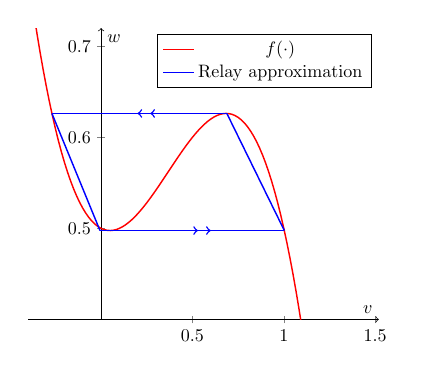
\begin{tikzpicture}[scale = 0.65]
  \begin{axis}[
    xmin=-.4,xmax=1.52,
    ymin=0.4,ymax=.72,
    axis lines=center,
    axis line style=->,
    xlabel={$v$},
    ylabel={$w$}
    ]
      \addplot[-] [color=red, style = thick] expression[domain=-0.45:1.2,samples=100]{-x^(3)+(1+0.1)*x^(2) - 0.1*x + 0.5}; 
      \addplot[-] [color=blue, style = thick] coordinates{(-.2693,0.6262) (.6883,.6262)};
            \addplot[<-] [color=blue, style = thick] coordinates{(.2693,0.6262) (.6883,.6262)};
            \addplot[<-] [color=blue, style = thick] coordinates{(.1993,0.6262) (.6883,.6262)};
      \addplot [color=blue, style = thick] coordinates{(.6883,0.6262) (1.003,.4976)};
      \addplot [color=blue, style = thick] coordinates{(-.2693,0.6262) (-.0061,.4976)};
      \addplot [-][color=blue, style = thick] coordinates{(-.0061,.4976) (1.003,.4976)};
      		\addplot [->][color=blue, style = thick] coordinates{(-.0061,.4976) (.6,.4976)};
            \addplot [->][color=blue, style = thick] coordinates{(-.0061,.4976) (.53,.4976)};
     % \addplot[-] [color=green, style = thick] expression[domain=-0.45:1.2,samples=100]{-y^(3)+(1+0.1)*y^(2) - 0.1*y + 0.5}; 
     \addlegendentry{$f(\cdot)$}
	 \addlegendentry{Relay approximation}
	\end{axis}
\end{tikzpicture}
	\caption{Nonlinearity and the ``relay" approximation}%
	\label{original_nonlinearity}%
\end{subfigure}
\caption{FitzHugh-Nagumo}
\label{fn}
\end{figure}

\vspace*{-.5cm}

\begin{figure}[h!]
\RawFloats
\centering
\begin{minipage}[t]{.45\textwidth}
\centering
\tikzstyle{block} = [draw,  rectangle,  minimum height=3em, minimum width=6em]
\tikzstyle{sum} = [draw,  circle, node distance=1cm]
\tikzstyle{input} = [coordinate]
\tikzstyle{output} = [coordinate]
\tikzstyle{pinstyle} = [pin edge={to-,thin,black}]

% The block diagram code is probably more verbose than necessary
\resizebox{4cm}{!}{%
\begin{tikzpicture}[auto, node distance=2cm,>=latex, scale = 0.5]
    % We start by placing the blocks
    \node at (0,3) (I_app) {$I_{app}$};
    %\node[input, name = I_app]{text};
    \node[sum, right of = I_app](sum_outer){};
    \node [block, right of = sum_outer] (inverse) {$-f^{-1}(\cdot)$};
    \node [output, right of = inverse] (output) {};
    \node [block, below of = inverse](linear_tf){\large $\frac{1}{s+\gamma}$};

    % Once the nodes are placed, connecting them is easy. 
    \draw [->] (sum_outer) --(inverse);
    \draw [->] (inverse) -- node [name=v] {$v$}(output);
    \draw [->](v) |- (linear_tf);
    \draw [->](linear_tf) -| node[anchor=south,pos=0.2] {$w$} 
    	node[pos=0.93]{-}(sum_outer);
    \draw [->](I_app)-- node[near end]{$+$} (sum_outer);
\end{tikzpicture}
}
	\captionof{figure}{High gain inversion}%
	\label{high_gain_inversion}%
\end{minipage}
\hspace{.5cm}
\begin{minipage}[t]{.45\textwidth}
\centering
\tikzstyle{block} = [draw,  rectangle,  minimum height=3em, minimum width=6em]
\tikzstyle{sum} = [draw,  circle, node distance=1cm]
\tikzstyle{input} = [coordinate]
\tikzstyle{output} = [coordinate]
\tikzstyle{pinstyle} = [pin edge={to-,thin,black}]
% The block diagram code is probably more verbose than necessary
\resizebox{4cm}{!}{%
\begin{tikzpicture}[auto, node distance=2cm,>=latex]
    % We start by placing the blocks
    \node at (0,3) (I_app) {$I_{app}$};
    %\node[input, name = I_app]{text};
    \node[sum, right of = I_app](sum_outer){};
    \node [block, right of = sum_outer] (inverse) {$f_{2}(\cdot)$};
    \node [output, right of = inverse] (output) {};
    \node [block, below of = inverse](linear_tf){\large $\frac{1}{s+\gamma}$};

    % Once the nodes are placed, connecting them is easy. 
    \draw [->] (sum_outer) --(inverse);
    \draw [->] (inverse) -- node [name=v] {$v$}(output);
    \draw [->](v) |- (linear_tf);
    \draw [->](linear_tf) -| node[anchor=south,pos=0.2] {$w$} 
    	node[pos=0.93]{+}(sum_outer);
    \draw [->](I_app)-- node[near end]{$-$} (sum_outer);
\end{tikzpicture}
}
      \captionof{figure}{$f_2(x) = -f^{-1}(-x)$}%
      \label{invert_y_axis}%
\end{minipage}
\end{figure}

\vspace{-1cm}

\begin{figure}[h!]
\begin{subfigure}[t]{0.45\textwidth}
\centering
\tikzstyle{block} = [draw,  rectangle,  minimum height=3em, minimum width=6em]
\tikzstyle{sum} = [draw,  circle, node distance=1cm]
\tikzstyle{input} = [coordinate]
\tikzstyle{output} = [coordinate]
\tikzstyle{pinstyle} = [pin edge={to-,thin,black}]

% The block diagram code is probably more verbose than necessary
\resizebox{4cm}{!}{%
\begin{tikzpicture}[auto, node distance=2cm,>=latex]
    % We start by placing the blocks
	
    \node [block] (inverse) {$f_3(\cdot)$};
    \node [output, right of = inverse] (output) {};
    \node [input, left of = inverse](input){};
    \node [block, below of = inverse](linear_tf){\large $\frac{1}{s+\gamma}$};

    % Once the nodes are placed, connecting them is easy. 
    \draw [-] (inverse) -- (output);
    \draw [->] (output) |- node[near start] {$\hat{v}$}(linear_tf);
    \draw [-] (linear_tf) -| node[near end] {$\hat{w}$} (input);
    \draw [->] (input) -- (inverse);

\end{tikzpicture}
}
\caption{Block diagram}
\end{subfigure}
\quad%
\begin{subfigure}[t]{.45\textwidth}
\centering
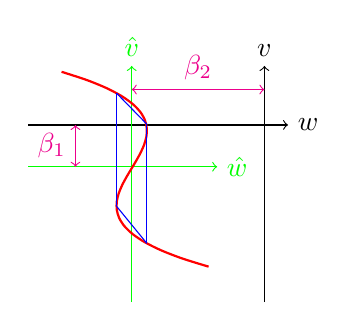
\begin{tikzpicture}[xscale=3,yscale=1.5]
  \newcommand\myscale{1};
  \draw[->] (-1*\myscale,0) -- (0.1*\myscale,0) node[right] {$w$};
  \draw[->] (0,-1.5*\myscale*\myscale) -- (0,.5*\myscale*\myscale) node[above] {$v$};
    \draw[->] [green](-1*\myscale,-.354) -- (-.2*\myscale,-.354) node[right] {$\hat{w}$};
  	\draw[->] [green](-.5619,-1.5*\myscale*\myscale) -- (-.5619,.5*\myscale*\myscale) node[above] {$\hat{v}$};
    \draw[<->][magenta](-.5619,.3) -- node[above]{$\beta_2$} (0,.3);
    \draw[<->][magenta](-.8,-.354) -- node[left]{$\beta_1$} (-.8,0);

% code for Mirror Image
\begin{scope}[xscale = -1,xshift=0cm]
  \begin{scope}[yscale=-1,yshift=0cm]
    \draw[scale=\myscale,domain=-.45:1.2,smooth,variable=\y,red, thick]  plot ({-(\y)^(3)+(1+0.1)*(\y)^(2) - 0.1*(\y) + 0.5},{\y});
    \draw[-,scale=\myscale,blue] (0.6262,-.2693) -- (0.6262,.6883);
    \draw[-,scale=\myscale,blue] (0.6262,.6883) -- (.4976,1.003);
    \draw[-,scale=\myscale,blue] (0.6262,-.2693) -- (.4976,-.0061);
    \draw[-,scale=\myscale,blue] (.4976,-.0061) -- (.4976,1.003);
  \end{scope}
  \end{scope}
\end{tikzpicture}
\caption{Nonlinearity in new co-ordinates, $f_3(\cdot)$}
\end{subfigure}
      \caption{Shift co-ordinate system to make relay symmetric, $I_{app}$ disappears. $\hat{w} = w + \beta_2$ and $\hat{v} = v + \beta_1$}%
      \label{shift1}%
\end{figure}\nopagebreak%
\begin{figure}[h!]
\RawFloats
\centering
\begin{minipage}[t]{.4\textwidth}
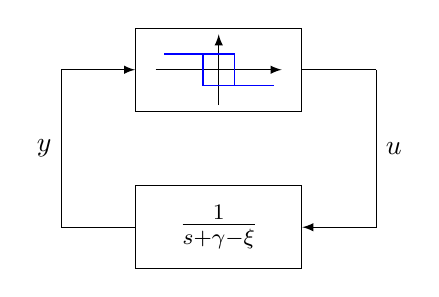
\begin{tikzpicture}[auto, node distance=2cm,>=latex]
\tikzstyle{block} = [draw,  rectangle,  minimum height=3em, minimum width=6em]
\tikzstyle{sum} = [draw,  circle, node distance=1cm]
\tikzstyle{input} = [coordinate]
\tikzstyle{output} = [coordinate]
\tikzstyle{pinstyle} = [pin edge={to-,thin,black}]   % We start by placing the blocks

\def\relay{
\tikz[remember picture,overlay]{
\draw[->] (-.8,0) -- (.8,0);
\draw[->] (0,-0.45)--(0,0.45);
\draw[blue] (0.7,-0.2)--(0.2,-0.2)--(0.2,0.2)--(-.7,.2);
\draw[blue] (-.2,.2)--(-.2,-.2)--(.2,-.2);
}}

    \node [block] (inverse) {};
    \node[] at (inverse) {\relay};
    \node [output, right of = inverse] (output) {};
    \node [input, left of = inverse](input){};
    \node [block, below of = inverse](linear_tf){\large $\frac{1}{s+\gamma-\xi}$};

    % Once the nodes are placed, connecting them is easy. 
    \draw [-] (inverse) -- (output);
    \draw [->] (output) |- node[near start] {$u$}(linear_tf);
    \draw [-] (linear_tf) -| node[near end] {$y$} (input);
    \draw [->] (input) -- (inverse);

\end{tikzpicture}
\captionof{figure}{Change of basis to use relay. $\hat{w}=y$ and $\hat{v} = \xi y + u$}
\label{fn_final_block}
\end{minipage}
\hspace{0.5cm}
\begin{minipage}[t]{.4\textwidth}\vspace{-2cm}\small
Following the steps from the Figures \ref{fn} to \ref{fn_final_block} allow the standard relay to be used to model the FitzHugh-Nagumo equations. The original variables can be recovered as: 
\begin{equation*}
\begin{cases}
v = \hat{v}-\beta_1 = \xi y + u - \beta_1 \\
w = \hat{w}-\beta_2 = y - \beta_2 \\
\end{cases}
\end{equation*}
\end{minipage}
\end{figure}


\newpage
The first step in replacing the cubic nullcline was to approximate it using a skewed relay. This involved selecting four points on the nullcline that represented the essential behaviour. The points chosen were: 
\begin{equation}
(-0.2693,0.6262),(0.6883,0.6262),(-0.0061,0.4976),(1.003,0.4976)
\end{equation}
These points now represent the nonlinear function $f(v)$. They undergo the transformations described in the above figures in order to convert them to a standard relay feedback system. To inverse the $f(v)$, each point was reflected about the $y=x$ line. Then they were reflected about the x-axis in order to swap the signs of the input signals. Next, they were reflected in the y-axis due to the minus sign. To centralise the relay about the origin, they points were shifted by $(\beta_2,\beta_1) = (-0.562,-0.354)$. $\xi$ was then chosen in order to get a standard relay --- multiply each point by the matrix S,:
\begin{equation}
S = \begin{bmatrix}
1 & 0 \\ -\xi & 1 
\end{bmatrix}  = \begin{bmatrix}
1 & 0 \\ 2 & 1 
\end{bmatrix}
\end{equation}  

This resulted in the four points being positioned at:
\begin{equation}
(0.0643,0.4917),(0.0643,-0.4917),(-0.0643,0.4917),(-0.0643,-0.4917)
\end{equation}

The skew matrix can be understood by considering the skewed relay as simply a relay with an extra loop as shown below. The equations show where the skew matrix comes from. Lumping the extra loop with the original plant gives the new system. 

\begin{figure}[h!]
\begin{tikzpicture}[auto, node distance=2cm,>=latex, scale = 1]
\draw [fill = white](1,1) rectangle (15,7);
\end{tikzpicture}
\caption{Skewed relay}
\end{figure}
\begin{figure}[h!]
\begin{tikzpicture}[auto, node distance=2cm,>=latex, scale = 1]
\draw [fill = white](1,1) rectangle (15,7);
\end{tikzpicture}
\caption{Maths}
\end{figure}

This is a standard relay with hysteresis limits $\epsilon = 0.0643$ and output $d = 0.4917$. The state-space representation of this system was thus:
\begin{align}
\dot{x} &= (\gamma-\xi)x + u = 2.5x + u \\
y &= x \\
u &= \begin{cases}
	               -0.4917 \text{ if } e > 0.0643 \text{ or } (e >-0.0643 \text{ and } u(t-) = 0.4917)\\
	                0.4917 \text{ if } e < -0.0643 \text{ or } (e < 0.0643 \text{ and } u(t-) = -0.4917)	              
	            \end{cases}
\end{align}

The original system is then recovered by:
\begin{align}
v&= \xi y + u - \beta_1 = -2y+u+0.354 \\
w&= y - \beta_2 = y + 0.562 
\end{align}

Using equation \ref{eq:2_3}, the time period was predicted to be 0.54 seconds. The local stability was tested using Theorem 3.1 of \cite{astrom1995}, with the $W$ matrix being equal to zero and hence having eigenvalues within the unit disk. 

\section{Three time scale burster}

In order to find the bistable range for the piece-wise linear model of the system, it requires us to find the two critical points at which the system changes from having only one equilibrium to two equilibriums. This was shown for the original model in Figure \ref{fig:ttsbursting_bistable_range}. 

\begin{figure}[h!]
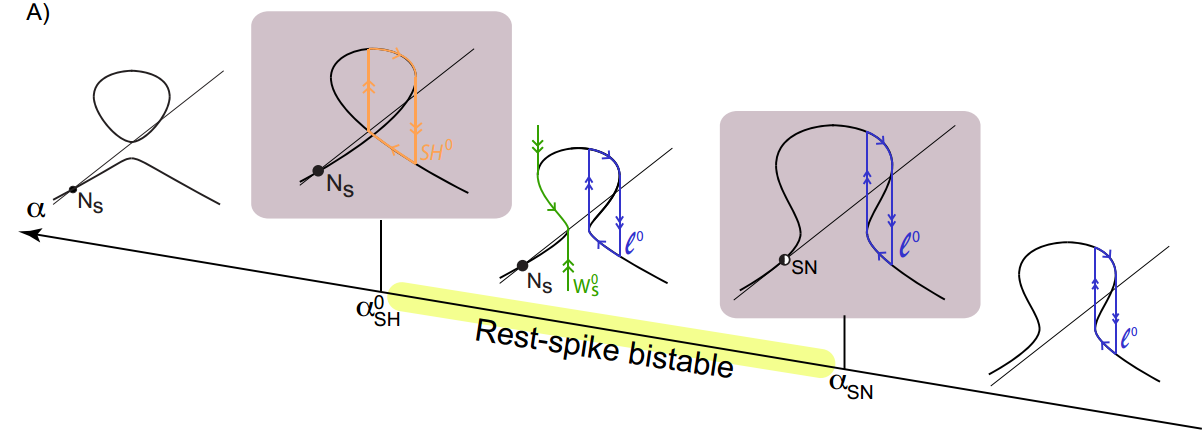
\includegraphics[width = 0.6\textwidth]{tts_bistable_range}
\caption{The bistable range for the $\alpha$ parameter.}
\end{figure}

The fast nullcline can be written as:
\begin{equation}
G(x_f, x_s, \alpha) = - x_f + \text{sign}\left(B\left(u+x_s + \tfrac{1}{2}\gamma x_f\right) + \beta x_f + \alpha \right)
\end{equation}
The extreme point of the lower branches are right when the sign $(\cdot)$ function changes from being 1 to $-1$. Since $x_f = -1$, this means: $B(u + x_s -\tfrac{1}{2}\gamma) -\beta + \alpha = 0$. This can be written as:
\begin{align}
\tfrac{1}{2}(u + x_s -\tfrac{1}{2}\gamma) - \beta + \alpha &= 0 \text{\hspace{2cm} if } -2< (u +  x_s -\tfrac{1}{2}\gamma)<0 \\
-\tfrac{1}{2}(u + x_s -\tfrac{1}{2}\gamma) - \beta + \alpha &= 0 \text{\hspace{2cm} if } 0< (u +  x_s -\tfrac{1}{2}\gamma)<2 \\
\end{align}
We are first concerned at which point the linear nullcline intersects the lower left hand branch of the fast nullcline. At that point, $x_f = -1$. This implies that $x_s = -1$  as well. This means:

\begin{equation}
\alpha_{max} = \beta + \tfrac{1}{2}(u-1-\tfrac{1}{2}\gamma)
\end{equation}

The two extreme points of the lower branch meet when we reach the peak of the bump, i.e $u + x_s - \tfrac{1}{2}\gamma = 0$. Thus:
\begin{equation}
\alpha_{min} = \beta
\end{equation}

\begin{figure}[h!]
\begin{tikzpicture}[auto, node distance=2cm,>=latex, scale = 1]
\draw [fill = white](1,1) rectangle (15,10);
\end{tikzpicture}
\caption{Fast nullcline branches.}
\end{figure}

\end{appendices}

\end{document}
